\documentclass[10pt,twocolumn]{article}
\usepackage[margin=0.75in]{geometry}
\usepackage{amsmath,amssymb,graphicx,booktabs,url}
\usepackage{cite}
\title{Message-Aware Low-Step Conversion of Dynamic Vision Graphs}
\author{Anonymous Author(s)}
\begin{document}
\maketitle
\begin{abstract}
Training-free ANN-to-SNN conversion has achieved low-step operation on convolutional and Transformer models, but dynamic vision graphs remain difficult because their neighbor selection and signed message aggregation amplify numerical errors. We first show that preserving neighbor indices and max-winner indices alone is insufficient: on a patch-grid dynamic Grapher, a structure-calibrated converter loses 33.37 percentage points of top-1 accuracy relative to its teacher, whereas restoring teacher features recovers nearly the entire gap. Guided by this diagnostic, we reformulate low-step conversion around the propagated message tensor and calibrate signed coding parameters to minimize message error on training data. Across three teacher seeds, message-aware calibration reduces the mean teacher gap from 33.37 to 4.77 points on Fashion-MNIST (85.71\% closure) and from 61.95 to 7.10 points on MNIST (88.54\% closure), while preserving the event budget. A paired bootstrap over 6,000 example-seed predictions gives a 95\% interval of +27.2 to +30.1 points for v2 versus v1 on Fashion-MNIST. Ablations show that resolution alone or offset alone is insufficient; the joint objective reduces message MSE by 82.19\% on Fashion-MNIST and 86.07\% on MNIST. The study identifies message fidelity, rather than discrete structure agreement alone, as the operative bottleneck in low-step graph conversion.
\end{abstract}

\section{Introduction}
Training-free conversion reuses trained artificial neural networks by replacing continuous activations with low-latency spiking or graded-spike codes. Recent methods reduce the number of time steps substantially on CNNs and Transformers, yet visual graph models pose a different challenge: every graph block constructs neighbors from current features and aggregates signed neighbor messages. Quantization error can therefore alter both continuous values and discrete graph decisions.

A natural hypothesis is that preserving discrete graph decisions is sufficient. We tested this hypothesis on a dynamic patch Grapher. Scale-based calibration produced substantial neighbor and winner disagreement, and teacher-feature oracles recovered almost all accuracy. However, a converter selected to improve structure agreement still trailed the teacher by 33.37 points on Fashion-MNIST. Restoring teacher features while retaining converted discrete decisions recovered 83.42\% mean accuracy, nearly matching the 83.60\% teacher mean. This result localizes the dominant error to the magnitude of the messages propagated between nodes.

We make three contributions. First, we provide an empirical diagnosis showing that discrete structure fidelity does not imply task fidelity in low-step graph conversion. Second, we formulate message-aware calibration, which fits signed coding parameters to minimize the Grapher message tensor on training data. Third, we validate the method across Fashion-MNIST and MNIST with three seeds each, matched event budgets, ablations, and a paired bootstrap interval.

\section{Related Work}
ANN-to-SNN conversion has progressed from rate-coded deep networks to calibration, quantized activation training, differential coding, and multi-threshold neurons \cite{cao2015spiking,rueckauer2017conversion,li2021calibration,huang2025dcgs}. These methods mainly target CNNs or Transformers. Graph conversion is less developed: fixed-text GCN conversion, tactile graph conversion, and point-cloud conversion either assume fixed topology, retrain the source with special activations, or replace max pooling before training \cite{onespike2025,pmsm2025,lan2023}. Direct-trained spiking graph networks, including SpikingGCN, Spiking PointNet, and related point-cloud models, optimize models from scratch rather than converting a pretrained dynamic graph [7, 8, 12]. Dynamic vision graphs such as ViG construct kNN from patch features and aggregate signed neighbor messages \cite{vig2022}. Efficient inference work uses sparse frame differences or event-driven graph updates, but does not solve low-step conversion of signed dynamic messages \cite{deltacnn2022,aegnn2022}. Our work connects these lines by treating the graph message tensor as the conversion target.

\section{Method}
Figure~\ref{fig:framework} summarizes the conversion pipeline. We use a patch-grid Grapher as a controlled dynamic vision graph. An image is split into patches, each patch is embedded as a node, and each Grapher block computes cosine-similarity kNN, applies a linear message map to neighbor-minus-center features, and max-pools the resulting signed messages per channel. The teacher is trained in floating point; conversion does not change its weights.

\begin{figure}[t]
\centering
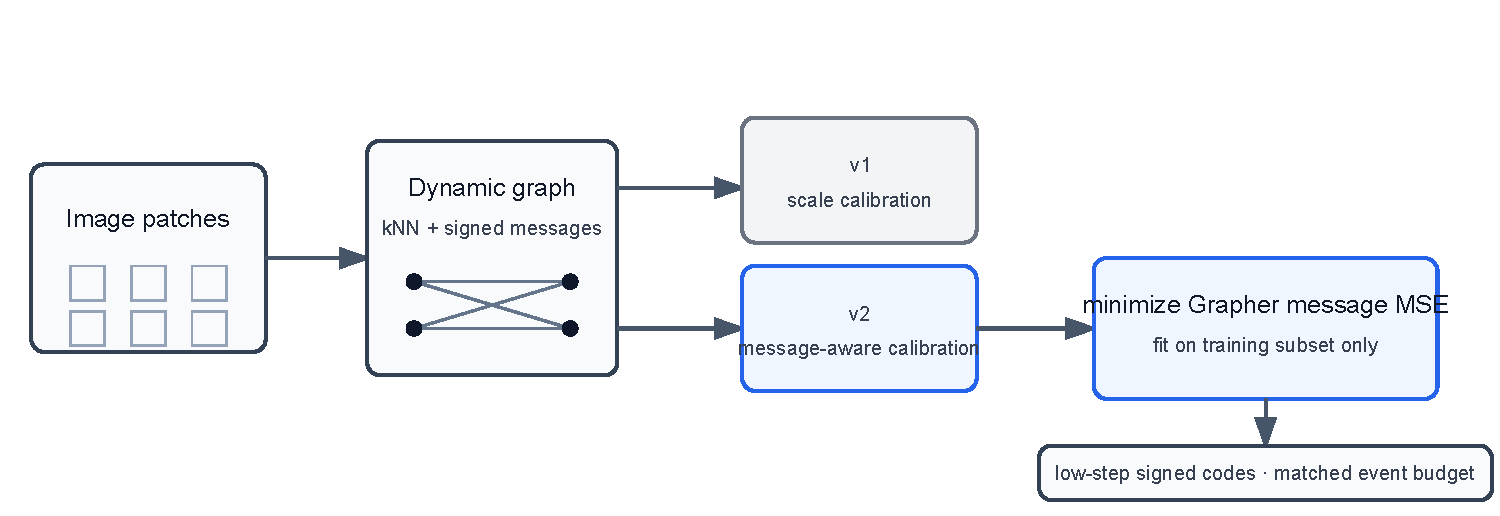
\includegraphics[width=\columnwidth]{figure1.pdf}
\caption{Conversion pipeline. The v1 control calibrates a scalar scale, whereas v2 selects coding parameters by minimizing Grapher message MSE.}
\label{fig:framework}
\end{figure}

For a tensor of coding levels $L$, signed uniform coding maps a value $v$ to
\begin{equation}
Q(v;s,o)=2\,\mathrm{round}\!\left(\frac{(\mathrm{clip}(v+o,-1,1)+1)s}{2}\right)/s-1-o ,
\end{equation}
where $s=L-1$ is the quantization scale and $o$ is an offset. We calibrate $s$ and $o$ on a fixed training subset. Let $h(X)$ denote teacher node features and $m(h)$ the aggregated signed message produced by the trained message layer and max readout. The calibration objective is
\begin{equation}
\min_{s,o}\; \mathbb{E}_{x\in\mathcal{C}}\left\|m(h(x))-m(Q(h(x);s,o))\right\|_2^2 .
\end{equation}
Only coding parameters are optimized. At inference, converted features are used for neighbor selection, winner selection, message aggregation, update, and readout. We count nonzero signed codes as graded events and compare methods at equal event budgets.

The diagnostic oracle variants replace selected converted components with teacher components: teacher features with converted indices/winners, teacher neighbor indices only, teacher winners only, and both. These variants are measurement instruments, not deployable methods.

\section{Experiments and Results}
\textbf{Setup.} We use Fashion-MNIST and MNIST with official train/test splits. A fixed 5,000-example training subset calibrates coding parameters, and a separate validation subset selects teacher checkpoints. Three teachers are trained with seeds 41, 42, and 43 for each dataset. Each final test has 2,000 examples per seed and is evaluated after calibration is frozen.

\textbf{Structure-only conversion fails.} On Fashion-MNIST, a scale-calibrated converter using signed uniform coding achieves 50.23\% mean accuracy, a 33.37-point teacher gap. On the frozen test, signed-uniform neighbor Jaccard is 0.065 and winner agreement is 0.488; signed multilevel coding similarly has 0.080 neighbor Jaccard and 0.521 winner agreement. Replacing encoded features with teacher features while retaining converted indices and winners raises accuracy to 83.42\%. Restoring teacher neighbor indices and winners reaches the teacher mean exactly. Thus the discrete decisions are useful diagnostics but are not sufficient to optimize.

\textbf{Message-aware conversion closes the gap.} Table~\ref{tab:main} reports the primary result. On Fashion-MNIST, message-aware calibration reaches 78.83\% mean accuracy, reducing the teacher gap to 4.77 points and closing 85.71\% of the v1 gap. On MNIST, it reaches 70.78\% versus a 77.88\% teacher, closing 88.54\% of the v1 gap. Message MSE falls by 82.19\% and 86.07\% on the two datasets. Event counts are matched within each dataset.

\begin{table}[t]
\centering
\caption{Frozen-test results. Accuracy is the mean over three seeds; event equality is checked within each dataset.}
\label{tab:main}
\begin{tabular}{lcccc}
\toprule
Dataset / Method & Teacher & v1 & v2 & Gap closure \\
\midrule
Fashion-MNIST & 83.60 & 50.23 & 78.83 & 85.71\% \\
MNIST & 77.88 & 15.93 & 70.78 & 88.54\% \\
\bottomrule
\end{tabular}
\end{table}

\textbf{Statistical and ablation evidence.} For Fashion-MNIST we saved all model predictions to compute a paired example-level difference between v2 and v1. Over 6,000 example-seed predictions, the mean improvement is 28.60 points with bootstrap 95\% interval [27.17, 30.08]. On the same dataset, scale-only calibration reaches 50.23\% and offset-only calibration reaches 38.85\%, whereas full message-aware calibration reaches 78.83\% for every seed. The result therefore depends on the objective, not merely on finer quantization or a shifted threshold.

\section{Discussion}
The initial structure-only hypothesis was falsified by the observed accuracy gap, while teacher-feature restoration recovered nearly all of it. This pattern distinguishes two error sources: discrete topology/winner changes and continuous message magnitude. Our results show that magnitude reconstruction can dominate practical accuracy under low-step graph conversion. Structure metrics remain useful diagnostics, but they should not be treated as substitutes for message or task fidelity.

The evidence is scoped to small patch-grid dynamic Graphers on two digit/apparel benchmarks, three seeds, and 2,000 test examples per seed. We report graded-event counts rather than hardware energy; no neuromorphic power measurement is claimed. Future work should test deeper dynamic vision backbones, additional visual datasets, and whether message-aware calibration transfers to other signed aggregation operators.

\section{Conclusion}
Low-step conversion of dynamic vision graphs is not solved by matching neighbor indices and max winners alone. Calibrating signed codes against the propagated message tensor closes 85.71\% and 88.54\% of the teacher gap on Fashion-MNIST and MNIST at matched event budgets, with consistent gains across all seeds. The study establishes message fidelity as a concrete target for training-free graph conversion and provides a diagnostic framework for separating structural and numerical failure modes.

\bibliographystyle{plain}
\bibliography{references}
\end{document}
